\documentclass[a4paper,11pt]{article}
%\usepackage{ngerman}
\usepackage[utf8]{inputenc}
\usepackage{geometry}
\usepackage{todonotes}
\usepackage{xcolor}
\usepackage{colortbl}
\usepackage{longtable}
\usepackage{array}
\usepackage{eurosym}
%\usepackage{hyperref}
\usepackage[colorlinks=true,breaklinks=true,linkcolor=kolor,urlcolor=kolor,citecolor=kolor]{hyperref}
\usepackage{graphicx}
%\usepackage{psfrag}
\usepackage{fancyhdr}
\usepackage{amssymb}
\usepackage{wrapfig}
%\usepackage[onehalfspacing]{setspace}
\usepackage{framed}
\usepackage{multirow}
%\usepackage{mdframed}
\usepackage{amsmath}
\usepackage{float}
\usepackage{blindtext}
%\usepackage{printlen}
%\usepackage{multirow}
%\usepackage{rotating}
%\usepackage{math}
\usepackage{titlesec}
\usepackage{etoolbox}
\usepackage{acronym}
\usepackage{pgfplots}
\usepackage{tikz}
\usepackage{pgf-pie}
\usepackage[utf8]{inputenc}
\usepackage{fancyhdr}
\usepackage[ruled,vlined,linesnumbered,noresetcount]{algorithm2e}



\geometry{left=2cm,top=2cm,right=2cm,bottom=2cm}


% define line line spacing
%\renewcommand{\baselinestretch}{1.2}

\renewcommand{\familydefault}{\sfdefault} %font
%\fontfamily{cmr}\selectfont %wie bsc


\definecolor{kolor}{RGB}{0,0,0}
\definecolor{maincol}{RGB}{178,201,225}
\definecolor{darkcol}{RGB}{0,78,155}




\setlength \abovecaptionskip{0pt}   % no spacing above caption

\setlength \parindent{0pt}  % no indent everywhere

% define citation style
\bibliographystyle{unsrt}

% define second level for `itemizing'
\renewcommand{\labelitemii}{-}


\renewcommand{\figurename}{Abbildung}
\renewcommand{\tablename}{Tabelle}
\renewcommand{\refname}{Referenzen}

\titleformat*{\section}{\huge\bfseries}
\titleformat*{\section}{\huge\bfseries}
\titleformat*{\subsection}{\LARGE\bfseries}
\titleformat*{\subsubsection}{\Large\bfseries}
\titleformat*{\paragraph}{\Large\bfseries}
\titleformat*{\subparagraph}{\Large\bfseries}



\makeatletter
\patchcmd{\ttlh@hang}{\parindent\z@}{\parindent\z@\leavevmode}{}{}
\patchcmd{\ttlh@hang}{\noindent}{}{}{}
\patchcmd{\@part}{\markboth{}{}}{\partmark{#1}}{}{} % \part in header
\makeatother
\begin{document}


% Deckblatt

\begin{center}

\thispagestyle{empty}

	
\includegraphics[width=8cm]{Images/uni-siegen-logo.png}
	\\
	\vspace*{1cm}
	\Large{Durchgeführt im Rahmen des}\\
	\Huge{\textbf{BMBF-Projekt: ELISE}}\\
	\vspace{1.0cm}
	\Huge{\textbf{Dokumentation der Projektarbeit}}\\
	\vspace{0.3cm}	
	\Large{Entwurf eines kompakten mikrocontrollergestützten Systems zur Emotionserkennung in einer Virtual-Reality-Umgebung}\\
\vspace{0.5cm}	
\Large{\textbf{WiSe 2017/2018 und SoSe 2018}}\\
\vspace{0.6cm}
\end{center}
	
\Large
\noindent
\underline{\textbf{Projektbetreuer:}}\\
\\
\noindent
\textbf{Medizinische Informatik und Mikrosystementwurf}\\
Prof. Dr. rer. nat. Rainer Brück\\
Dr.-Ing. Armin Grünewald\\
M.Sc. David Krönert\\
M.Sc. Tanja Eiler\\

\noindent
\textbf{Forschungsgruppe für Mustererkennung}\\
Prof. Dr.-Ing. Marcin Grzegorzek\\
M.Sc. Frédéric Li\\
\vspace*{1.2cm}

\noindent
\underline{\textbf{Projektteilnehmer:}}\\
\\
\noindent
Artur Piet (Sprecher der Projektgruppe)\\
Jonas Pöhler (Stellv. Sprecher der Projektgruppe)\\
Arnaud Eric Toham Waffo\\
Boris Kamdem\\
Kevin Orth\\
Meryem Dural\\
Minas Michail\\


% Inhaltsverzeichnis
\newpage
\renewcommand{\contentsname}{Inhaltsverzeichnis}
\tableofcontents
\clearpage


% Zusammenfassung/Abstract
\newpage

\section*{Begrifflichkeiten}
\addcontentsline{toc}{section}{Begrifflichkeiten}

\noindent
\todo[inline]{Kurze Beschreibung der verwendeten Begriffe/Abkürzungen}



% 1
\newpage
\section{Einleitung} \label{einleitung-sec}
\todo[inline]{Minas}



% Unterkapitel 1.1
\subsection{Hintergrund und Motivation} \label{hintergrund-subsec}






% Unterkapitel 1.2
\subsection{ELISE Projektbeschreibung} \label{elise-subsec}






% Unterkapitel 1.3
\subsection{Gliederung dieser Dokumentation} \label{gliederung-subsec}



% Unterkapitel 1.4
\subsection{Anhang}  \label{anhang-subsec}






% 2
\newpage
\section{Organisation} \label{organisation-sec}

\noindent
\todo[inline]{Artur \\
- Gliederung muss noch gemacht werden!}



% 3
\newpage
\section{Grundlagen} \label{grundlagen-sec}
\todo[inline]{Minas}



% Unterkapitel 3.1
\subsection{Definition von Emotionen} \label{definition-emotionen-sec}




% Unterkapitel 3.2
\subsection{Virtual Reality (VR)} \label{grund-vr-subsec}




% Unterkapitel 3.3
\subsection{Sensoren und biophysiologische Signale zur Emotionserkennung} \label{grund-sensoren-subsec}



% Unterkapitel 3.1.1
\subsubsection{Körpertemperatur-Sensor} \label{grund-temp-subsubsec}




% Unterkapitel 3.1.2
\subsubsection{Blood Volume Pulse-Sensor (BVP)} \label{grund-bvp-subsubsec}




% Unterkapitel 3.1.3
\subsubsection{Messen der Sauerstoffsättigung (SpO2)} \label{grund-spo2-subsubsec}




% Unterkapitel 3.1.4
\subsubsection{Galvanic Skin Response (GSR)} \label{grund-gsr-subsubsec}




% Unterkapitel 3.1.5
\subsubsection{Elektroenzephalografie (EEG)} \label{grund-eeg-subsubsec}




% Unterkapitel 3.1.6
\subsubsection{Elektrookulografie (EOG)} \label{grund-eog-subsubsec}




% Unterkapitel 3.1.7
\subsubsection{Analog/Digital-Wandler} \label{grund-ad-wandler-subsubsec}




% Unterkapitel 3.4
\subsection{Kommunikation} \label{grund-kommunikation-subsec}








% 4
\newpage
\section{State-of-the-Art Analyse} \label{soa-sec}
\todo[inline]{Jonas \\
- Gliederung muss noch gemacht werden!}






% 5
\newpage
\section{Systementwurf und Konzept} \label{systementwurf-sec}
\todo[inline]{Kevin}



% Unterkapitel 5.1
\subsection{Anforderungen} \label{anfoderungen-subsec}





% Unterkapitel 5.2
\subsection{Konzept} \label{konzept-subsec}







% Unterkapitel 5.3
\subsection{Hardwareauswahl} \label{hardwareauswahl-subsec}



% Unterkapitel 5.3.1
\subsubsection{Auswahlkriterien} \label{auswahlkriterien-subsubsec}






% Unterkapitel 5.3.2
\subsubsection{Festlegung der genutzten Hardware} \label{festlegung-subsubsec}










% Unterkapitel 5.4
\subsection{Hardwarearchitektur} \label{hardwarearchitektur-subsec}



% Unterkapitel 5.4.1
\subsubsection{GSR-Sensor} \label{gsr-subsubsec}






% Unterkapitel 5.4.2
\subsubsection{Temperatur-Senosr} \label{temp-subsubsec}








% Unterkapitel 5.4.3
\subsubsection{Pulsoximeter} \label{pulsoximeter-subsubsec}








% Unterkapitel 5.4.4
\subsubsection{EEG} \label{eeg-subsubsec}








% Unterkapitel 5.4.5
\subsubsection{EOG} \label{eog-subsubsec}








% Unterkapitel 5.4.6
\subsubsection{Datenübertragung} \label{datenuebertragung-subsubsec}










% Unterkapitel 5.5
\subsection{Programmierung} \label{programmierung-subsec}







% Unterkapitel 5.6
\subsection{Aufnahme der übertragenen Daten} \label{aufnahme-daten-subsec}









% 6
\newpage
\section{Realisierung} \label{realisierung-sec}
\todo[inline]{Jonas \\
- Gliederung muss noch gemacht werden!}




% 7
\newpage
\section{Emotionsinduktion} \label{emotionsinduktion-sec}
\todo[inline]{Meryem}


% Unterkapitel 7.1
\subsection{Ablauf} \label{ablauf-subsubsec}





% Unterkapitel 7.2
\subsection{Fragebogen} \label{fragebogen-subsec}







% Unterkapitel 7.3
\subsection{Szenarien} \label{szenarien-subsec}



% Unterkapitel 7.3.1
\subsubsection{Glück} \label{glueck-subsubsec}






% Unterkapitel 7.3.2
\subsubsection{Langeweile} \label{langeweile-subsubsec}








% Unterkapitel 7.3.3
\subsubsection{Frustration} \label{frust-subsubsec}







% 8
\newpage
\section{Messreihen} \label{messreihen-sec}
\todo[inline]{Kevin}



% Unterkapitel 8.3.1
\subsection{Erste Messreihe} \label{erste-messreihe-subsec}






% Unterkapitel 8.3.2
\subsection{Zweite Messreihe} \label{zweite-messreihe-subsec}








% Unterkapitel 8.3.3
\subsection{Dritte Messreihe} \label{dritte-messreihe-subsec}







% 9
\newpage
\section{Mustererkennung} \label{mustererkennung-sec}
\todo[inline]{Artur}



% Unterkapitel 9.1
\subsection{Grundlagen der Mustererkennung} \label{grundlagen-mustererkennung-subsec}


Mustererkennung (enlg. ``pattern recognition") ist ein Unterthema des machinellen Lernens.
Das Ziel besteht darin, automatisierte Systeme zu entwerfen, die hoch abstrakte Muster in Daten erkennen können.
Konkret heißt dies, dass man Maschinen beibringen möchte komplexer Aufgaben zu lösen, welche vom Menschen nahzu mühlelos und natürlich erledigt werden können.
Typische Beispiele für die zahlreichen Anwendungsbereiche sind die Objekterkennung, Spracherkennung sowie die Erkennung und Verfolgung in Bildern. 
Die Emotionserkennung ist ein Anwendungsbereich der Mustererkennung.
Die Hauptidee hinter der Lösung eines Mustererkennung-Problems ist es, dieses als Klassifikationsproblem zu übersetzen, wobei die zu erkennende Mustern die unterschiedliche Klassen bilden. 
Die vom Mustererkennungs-System eingegebenen Daten werden dann verarbeitet und der ``am nächsten liegenden" Klasse zugeordnet.
Beispielsweise können bei der Emotionserkennung die Eingangsdaten Bilder oder physiologische Signale sein, die in verschiedene Klassen eingeteilt werden, welche jeweils einer Emotion entsprechen. \\

Ein wichtiger Teil eines jeden Mustererkennung-Problems ist der Lernansatz, mit welchem die Maschine lernen soll die Muster in den Daten zu erkennen. 
Traditionell werden zwei Ansätze verwendet:

\begin{itemize}%[noitemsep]
  \item \underline{Überwachter Lernansatz:}
  Dieser Ansatz kann nur verwendet werden, wenn vor der Verarbeitung der Daten ein Datenbeschriftungsschritt durchgeführt wurde.
  In diesem Schritt wird jedem Element des Datensatzes ein Etikett (engl. ``label") zugewiesen, das angibt, welcher Klasse der jeweilige Datenpunkt zugeordnet werden kann.
  Die zusätzlichen Informationen, die die Etiketten liefern, werden als Grundlage verwendet, um sie mit der Vorhersage des Systems zu vergleichen und zu korrigieren, wenn sie nicht gleich sind.

  \item \underline{Unüberwachter Lernansatz:}
  Dieser Ansatz wird verwendet, wenn keine Etiketten für die Daten vorhanden sind.
  Unüberwachte Lerntechniken zielen darauf ab, der Maschine beizubringen, Muster in den Daten selbst zu finden. 
  Sie werden meist verwendet, um Einblicke in Daten zu erhalten, deren Struktur unbekannt ist.
\end{itemize} %\vspace{0.5cm}


Überwachtes Lernen liefert aktuell weit bessere Ergebnisse, jedoch ist die Beschriftung mit Etiketten der Daten nicht immer einfach oder teilweise sogar gar nicht möglich (z.B. wenn die Datenmenge sehr groß ist oder wenn Unsicherheit über die Vergabe der Etiketten besteht).
Aus diesem Grund wächst das Interesse an unüberwachter Lernansätzen.
Diese Ansätze sind jedoch schwierig zu benutzen, da sie eine große Menge an Daten voraussetzen.
Kompromisse sind mit semi-überwachten Lernansätzen möglich, bei denen die Daten für einen Teil des Datensatzes (aber nicht für den ganzen Datensatz) mit Etiketten beschriftet und damit bekannt sind.
In diesem Fall kann eine Mischung aus überwachten und Unüberwachter Techniken angewendet werden \cite{Zhu2008}.


% Unterkapitel 9.2
\subsection{Emotion Recognition Chain} \label{emotion-recogniton-chain-subsec}

Die Emotion Recognition Chain (ERC) besteht aus fünf Hauptschritten: 
Datenerfassung, Vorverarbeitung, Segmentierung, Merkmalsextraktion und Klassifizierung (vgl. Abb. \ref{fig:erc}).
In den folgenden Unterkapiteln wird für jeden Schritt eine allgemeine Erklärung gegeben. \\

\todo[inline]{Artur: Need to update the erc image}

\begin{figure}[h]
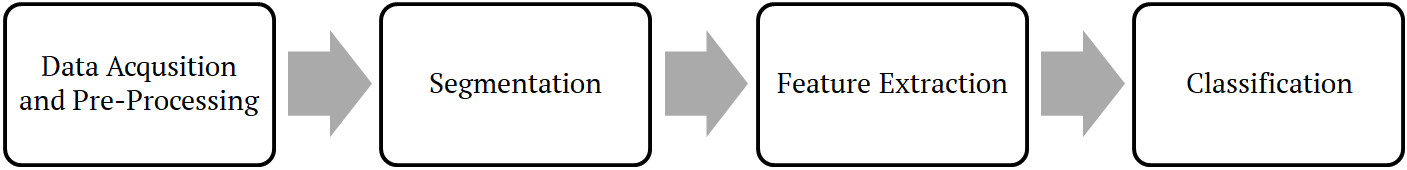
\includegraphics[width=\textwidth]{Images/erc.png} 
\vspace{-0.3cm} 
\caption{Emotion Recognition Chain: Zeitreihen-Datensätze werden von tragbaren Sensoren aufgenommen (Datenerfassung) und vorverarbeitet (Vorverarbeitung). Die Daten werden dann in Segmente unterteilt (Segmentierung), aus denen Merkmale extrahiert werden (Merkmalsextraktion). Mit den gewonnenen Merkmalen wird schließlich ein Klassifikator trainiert und anschließend dessen Ergebnisse bewertet (Klassifikation).}
\label{fig:erc} 
\end{figure} 
%\vspace{0.5cm}


% Unterkapitel 9.2.1
\subsubsection{Datenerfassung} \label{datenerfassung-subsubsec}


\todo[inline]{Artur: Später mit dem Rest der Dokumentation abstimmen.}


Dieser Schritt der ERC beinhaltet die Auswahl sowie den Aufbau der Sensoren, die Messreihendurchführung um Daten zu erhalten und Etikett-Beschriftungstechniken.
All diese Details sind wichtig für die Emotionserkennung, damit relevante und möglichst fehlerfreie Daten von Versuchspersonen für die verschiedenen emotionalen Zustände gewonnen werden können.
Dies ist besonders wichtig, da der Datenerfassungsschritt der erste in der ERC ist und die Ergebnisse aller folgenden Schritte direkt von der Qualität des Datensatzes abhängen. \\



% Vorverarbeitung, um die Daten von Rauschen zu reinigen.

% Unterkapitel 9.2.2
\subsubsection{Vorverarbeitung} \label{vorverarbeitung-subsubsec}


Normalisierungstechniken wurden auf dem gesamten Datensatz angewendet. 
Wir haben insbesondere die Standardnormalisierung verwendet, welche den Mittelwert der Daten auf Null setzt und die Einheitsvarianz ergibt \cite{grus15}. 
Die Formel für die Standardnormierung lautet:
\begin{equation} 
\Large{ {x'={\frac {x-{\overline {x}}}{\sigma }}} } 
\label{equ:norm} \end{equation} %\vspace{0.5cm}

wobei $ x $ ein Datenpunkt eines Sensorkanales, $ \overline{x} $ ist der Durchschnitt der Gesamtheit für diesen Sensorkanal und $ \sigma $ ist die entsprechende Standardabweichung.

% Unterkapitel 9.2.3
\subsubsection{Segmentation} \label{segmentation-subsubsec}


Ziel dieses Schrittes ist es, Teile von Daten zu identifizieren, welche wichtige Informationen über die zu erkennenden Emotionen enthalten. 
Dies geschieht durch Filtern der Daten und Ausschließen von Segmenten, die für das Klassifizierungsproblem nicht relevant sind.
Zusätzlich wird die zu verarbeitende Datenmenge reduziert, indem Segmente eines Zeitfensters fester Größe aus den Daten extrahiert werden.
Diese Vorgeheisweise ist heute in der Praxis besonders wichtig, da sonst hardwarebedingte Einschränkungen die zu verarbeitende Datenmenge begrenzen können. \\


In dieser Projektarbeit wurde ein Schiebefensteransatz (engl. ``sliding window approach'') verwendet. 
Ziel der Methode ist die Segmentierung der vorhandenen Daten in kleinere Einheiten, um die Merkmalsextraktion sowie die anschließende Klassifizierung zu vereinfachen oder gar erst zu ermöglichen.
Die Länge des Zeitfensters (engl. ``time window'') und des Gleitschritts (engl. ``sliding stride'') sind zu bestimmende Parameter (und werden auch als ```Hyperparameter'' bezeichnet), wobei sich das Zeitfenster auf die feste Größe pro extrahiertem Segment und der Gleitschritt auf die Lücke zwischen dem Beginn jedes Zeitfensters bezieht.
Es ist zu beachten, dass sich aufeinanderfolgende Zeitfenster überlappen können, sobald der definierte Schritt kleiner als das Zeitfenster ist. \\


Die Daten werden auf Zeitstempel-Ebene mit Etiketten beschriftet, basierend auf den von der jeweiligen Versuchsperson ausgefüllten Fragebögen. 
Jedem Zeitfenster wird ein Etikett zugeordnet, welches das dominaten (d.h. am meisten vohandene) Etikett der im Fenster enthaltenen Zeitstempel basiert. Es wird davon ausgegangen, dass jedes Zeitfenster nur von einer Emotion belegt ist. \\


\begin{figure}[h]
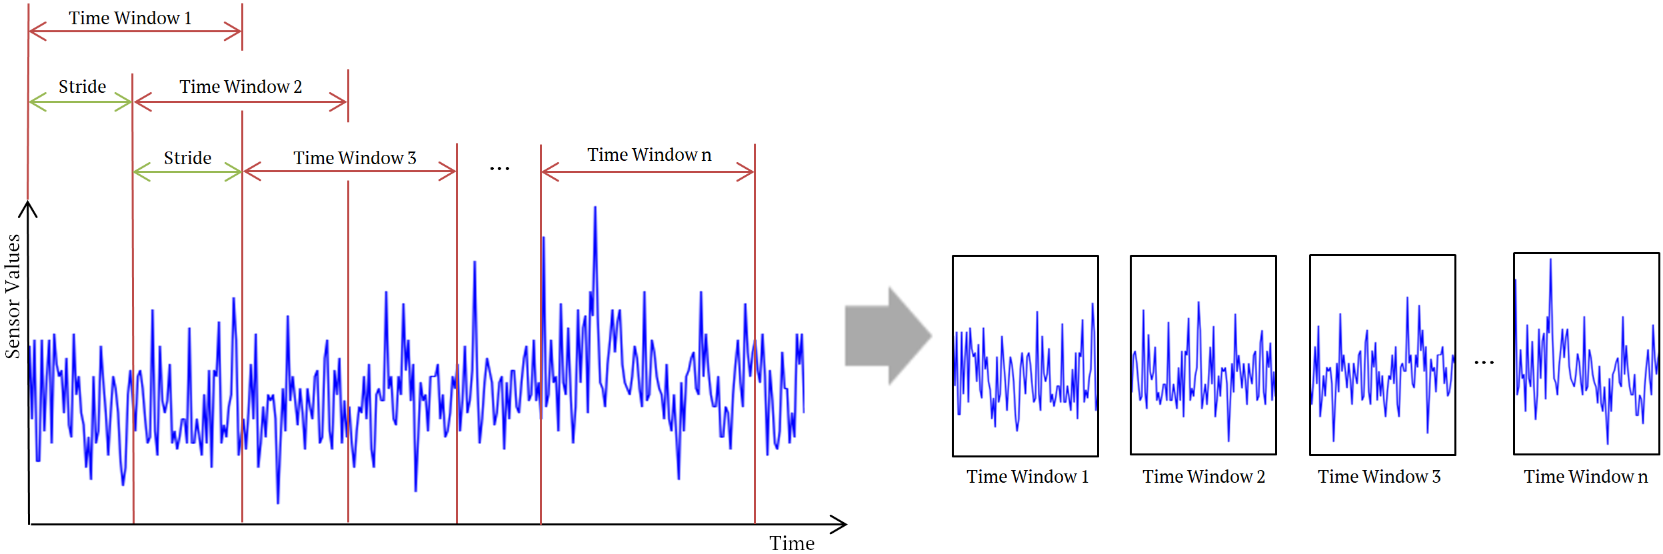
\includegraphics[width=\textwidth]{Images/segmentation.png} 
\caption{\small{Schiebefenster-Segmentierung: Die Daten werden durch ein Fenster fester Größe in kleinere Segmente aufgeteilt. Das Fenster wird mit einem festen Gleichschritt geschoben, um den aufeinanderfolgend Daten-Zeitfenster zu erhalten. }}
\end{figure} 

% Unterkapitel 9.2.4
\subsubsection{Merkmalsextraktion} \label{merkmalsextraktion-subsubsec}






% Unterkapitel 9.2.5
\subsubsection{Klassifikation} \label{klassifikation-subsubsec}








% Unterkapitel 9.3
\subsection{Merkmalsextraktion für Emotionserkennung} \label{merkmalsextraftion-emotionserkennung-subsec}



% Unterkapitel 9.3.1
\subsubsection{Hand-gefertigte Merkmale} \label{hc-features-subsubsec}






% Unterkapitel 9.3.2
\subsubsection{Codebook Approach} \label{codebook-approach-subsubsec}









% 10
\newpage
\section{Ergebnisse} \label{ergenisse-sec}
\todo[inline]{Artur}



% Unterkapitel 10.1
\subsection{Ergebnisse der hand-gefertigten Merkmale} \label{ergebnisse-hc-features-subsec}









% Unterkapitel 10.2
\subsection{Ergebnisse des Codebook Approach} \label{ergebnisse-codebook-approach-subsec}









% Unterkapitel 10.3
\subsection{Analyse der Ergebnisse} \label{analyse-subsec}











% 11
\newpage
\section{Zusammenfassung und Ausblick} \label{ende-sec}
\todo[inline]{Jonas}



% Unterkapitel 11.1
\subsection{Zusammenfassung} \label{zusammenfassung-subsec}








% Unterkapitel 11.2
\subsection{Fazit} \label{fazit-subsec}









% Unterkapitel 11.3
\subsection{Ausblick} \label{ausblick-subsec}











% List of Figures
\newpage 
\renewcommand{\listfigurename}{Abbildungsverzeichnis}
\addcontentsline{toc}{section}{Abbildungsverzeichnis}
\listoffigures


% List of Tables
\newpage
\renewcommand{\listtablename}{Tabellenverzeichnis}
\addcontentsline{toc}{section}{Tabellenverzeichnis}
\listoftables


% Anhang
\newpage
\section*{Anhang}
\addcontentsline{toc}{section}{Anhang}
%\input{8-WorkPlan/section}


% Referenzen
\newpage
\bibliographystyle{plain}
\bibliography{References/artur,References/marcin}

\end{document}